% \begin{frame}{Sélection}
% 	TODO	
% \end{frame}

\begin{frame}{Évaluation (Aptitude)}

% TODO: Faire un gros check up de cette formule notamment pour les valeurs minimale et maximale.

  \begin{block}{Overview}
    \begin{itemize}
      \item Détermine à quelle point un individu est une bonne solution
      \item Modélisation la plus liée au problème
      \item Aucune hypothèse n'est faite sur cette fonction
    \end{itemize}
  \end{block}

  \begin{align}
    f(\mathcal{C}) &= \frac{1}{2} \left(
      \frac{\Gamma(\mathcal{C}) - \Gamma(\mathcal{C}_{\textrm{min}})}
      {\Gamma(\mathcal{C}_{\textrm{max}}) - \Gamma(\mathcal{C}_{\textrm{min}})}
      +
      \frac{\mathcal{L(C)} - \mathcal{L(C_{\textrm{min}})}}
      {\mathcal{L(C_{\textrm{max}})} - \mathcal{L(C_{\textrm{min}})}}\right)\\
                   &= \frac{1}{2} \left(\Gamma(\mathcal{C})
        +\frac{\mathcal{L(C)} - \mathcal{L(C_{\textrm{min}})}}
        {\mathcal{L(C_{\textrm{max}})} - \mathcal{L(C_{\textrm{min}})}}\right)
  \end{align}
  \pnote{
    Partie la plus liée au problème. les autres points sont assez communs d'un probleme multi-objectifs à l'autre
  }    
  \pnote{
    Utilisation des valeurs extremes pour simplifier les calculs
  }
  \pnote{
    Aucune hypothèse n'est faite sur cette fonction (convexité, continuité, etc.)
  }
\end{frame}

\begin{frame}{Mutation}
	\begin{block}{Mutation polynomiale}
		\begin{itemize}
			\item $p_m$: Probabilité que la mutation se produise (0.2)
			\item $\eta_m$: Index de la distribution (Valeur recommandée: 20)
		\end{itemize}
	\end{block}
	\begin{figure}
		\centering
		\includegraphics[scale=.5]{figures/mutation_eta.pdf}
	\end{figure}

	\pnote{
		- Paramètre recommandée
	}
\end{frame}

\begin{frame}{Crossover}
	\begin{figure}[ht]
	  \centering
	  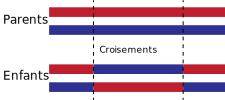
\includegraphics[scale=1]{../img/crossover.pdf}
	\end{figure}
	\pnote{
		- Paramètres recommandée par Sean Luke. Essentials of Metaheuristics.
	}
	\pnote{
		- A permis d'obtenir des résultats.
	}
	\pnote{
		- Principal concurrence avec un point simple mais si les allèles ne sont pas mises au hasard
		les premières sont souvent plus sélectionnées que les autres.
	}
\end{frame}